% XeLaTeX document
\documentclass[12pt,a4paper]{article}

% Редактируем: конфигурация, личные настройки: имя, название предмета и пр. для титульной страницы и метаданных документа здесь
\newcommand{\university}{Санкт-Петербургский политехнический университет Петра Великого}
\newcommand{\faculty}{Институт прикладной математики и механики}
\newcommand{\department}{Высшая школа прикладной математики и вычислительной физики}
\newcommand{\city}{Санкт-Петербург}
\newcommand{\num}{ № 1}
\newcommand{\docname}{Отчёт по лабораторной работе}
\newcommand{\subject}{Название предмета}
\newcommand{\tutorname}{С. Г. Попов}
\newcommand{\studentname}{В. А. Тюльпин}
\newcommand{\group}{3630201/60101}

% Не редактируем: используемые пакеты
% настройка кодировки, шрифтов и русского языка
\usepackage[utf8]{inputenc}
\usepackage[T2A]{fontenc}
\usepackage[russian]{babel}

% рабочие ссылки в документе
\usepackage{hyperref}

% графика
\usepackage{graphicx}

% поворот страницы
\usepackage{pdflscape}

% качественные листинги кода
\usepackage{minted}

% отключение копирования номеров строк из листинга, работает не во всех просмотрщиках (в Adobe Reader работает)
\usepackage{accsupp}
\newcommand\emptyaccsupp[1]{\BeginAccSupp{ActualText={}}#1\EndAccSupp{}}
\let\theHFancyVerbLine\theFancyVerbLine
\def\theFancyVerbLine{\rmfamily\tiny\emptyaccsupp{\arabic{FancyVerbLine}}}

% библиография
\bibliographystyle{templates/gost-numeric.bbx}
\usepackage{csquotes}
\usepackage[parentracker=true,backend=biber,hyperref=false,bibencoding=utf8,style=numeric-comp,language=auto,autolang=other,citestyle=gost-numeric,defernumbers=true,bibstyle=gost-numeric,sorting=ntvy,]{biblatex}

% установка полей
\usepackage{geometry}

% нумерация картинок по секциям
\usepackage{chngcntr} 

% для заголовков
\usepackage{caption} 
\usepackage{titlesec}
\usepackage[dotinlabels]{titletoc}

% разное для математики
\usepackage{amsmath, amsfonts, amssymb, amsthm, mathtools}

% водяной знак на документе, см. main.tex
\usepackage[printwatermark]{xwatermark} 

% Не редактируем: параметры используемых пакетов и не только
% настройки polyglossia
\setdefaultlanguage{russian}
\setotherlanguage{english}

% локализация
\addto\captionsrussian{
  \renewcommand{\figurename}{Рисунок}%
  \renewcommand{\partname}{Глава}
  \renewcommand{\contentsname}{\centerline{Содержание}}
  \renewcommand{\listingscaption}{Листинг}
}

% основной шрифт документа
\setmainfont{CMU Serif}

% перечень использованных источников
\addbibresource{refs.bib}

% настройка полей
\geometry{top=2cm}
\geometry{bottom=2cm}
\geometry{left=2cm}
\geometry{right=2cm}
\geometry{bindingoffset=0cm}

% настройка ссылок и метаданных документа
\hypersetup{unicode=true,colorlinks=true,linkcolor=red,citecolor=green,filecolor=magenta,urlcolor=cyan,        		       
    pdftitle={\docname},   	    
    pdfauthor={\studentname},      
    pdfsubject={\subject},      		        
    pdfcreator={\studentname}, 	       
    pdfproducer={Overleaf}, 		     
    pdfkeywords={\subject}
}

% настройка подсветки кода и окружения для листингов
\usemintedstyle{colorful}
\newenvironment{code}{\captionsetup{type=listing}}{}

% шрифт для листингов с лигатурами
\setmonofont{FiraCode-Regular.otf}[
    Path = templates/,
    Contextuals=Alternate
]

% оформления подписи рисунка
\captionsetup[figure]{labelsep = period}

% подпись таблицы
\DeclareCaptionFormat{hfillstart}{\hfill#1#2#3\par}
\captionsetup[table]{format=hfillstart,labelsep=newline,justification=centering,skip=-10pt,textfont=bf}

% путь к каталогу с рисунками
\graphicspath{{fig/}}

% Внесение titlepage в учёт счётчика страниц
\makeatletter
\renewenvironment{titlepage} {
 \thispagestyle{empty}
}
\makeatother

\counterwithin{figure}{section}
\counterwithin{table}{section}

\titlelabel{\thetitle.\quad}

% для удобного конспектирования математики
\mathtoolsset{showonlyrefs=true}
\theoremstyle{plain}
\newtheorem{theorem}{Теорема}[section]
\newtheorem{proposition}[theorem]{Утверждение}
\theoremstyle{definition}
\newtheorem{corollary}{Следствие}[theorem]
\newtheorem{problem}{Задача}[section]
\theoremstyle{remark}
\newtheorem*{nonum}{Решение}

% настоящее матожидание
\newcommand{\MExpect}{\mathsf{M}}

% объявили оператор!
\DeclareMathOperator{\sgn}{\mathop{sgn}}

% перенос знаков в формулах (по Львовскому)
\newcommand*{\hm}[1]{#1\nobreak\discretionary{} {\hbox{$\mathsurround=0pt #1$}}{}} 


% водяной знак для обозначения статуса документа
% \newwatermark[allpages,color=red!5,angle=45,scale=3,xpos=0,ypos=0]{DRAFT}
\begin{document}
% Не редактируем: Титульная страница (формируется автоматически из заданной конфигурации)
\begin{titlepage}	% начало титульной страницы

	\begin{center}		% выравнивание по центру

		\large \university \\
		\large \faculty \\
		\large \department \\[6cm]
		% название института, затем отступ 6см
		
		\huge \subject \\[0.5cm] % название работы, затем отступ 0,5см
		\large \docname \num \\[5.1cm]
		% \large Тема работы\\[5cm]

	\end{center}


	\begin{flushright} % выравнивание по правому краю
		\begin{minipage}{0.25\textwidth} % врезка в половину ширины текста
			\begin{flushleft} % выровнять её содержимое по левому краю

				\large\textbf{Работу выполнил:}\\
				\large \studentname \\
				\large {Группа:} \group \\
				
				\large \textbf{Преподаватель:}\\
				\large \tutorname

			\end{flushleft}
		\end{minipage}
	\end{flushright}
	
	\vfill % заполнить всё доступное ниже пространство

	\begin{center}
	\large \city \\
	\large \the\year % вывести дату
	\end{center} % закончить выравнивание по центру

\end{titlepage} % конец титульной страницы

\vfill % заполнить всё доступное ниже пространство


% Не редактируем: Страница содержания (формируется автоматически из section, subsection и пр., указанных в content.tex)
% Содержание
\tableofcontents
\newpage



% Редактируем: всё остальное: вступление, др. этапы, заключение, приложение
\section*{Постановка задачи}
Необходимо сделать нормальный шаблон для отчётов в Политехе. Структура отчётов может быть разной, зависит от требования преподавателя, поэтому файл content.tex отдельно выделен от всех других в шаблоне и не делится на подчасти.
\addcontentsline{toc}{section}{Постановка задачи}

\section{Программа работы}

\section{Теоретическая информация}

\section{Ход выполнения работы}

\subsection{Список}

\begin{itemize}
\item первый элемент списка
\item второй элемент списка
\end{itemize}


\subsection{Картинка}

\begin{figure}[H]
	\begin{center}
		\includegraphics[scale=0.7]{sample}
		\caption{название картинки} 
		\label{pic:pic_name} % название для ссылок внутри кода
	\end{center}
\end{figure}

Текст без отступа (следует за вставкой)

Новый параграф

\noindent Новый параграф с принудительно выключенным отступом


\subsection{Таблица}

\begin{table}[H]
	\caption{ Название таблицы}
	\begin{center}
		\begin{tabular}{|l|l|}
			\hline
			top left & top right\\ \hline
			bot left & bot right\\ \hline
		\end{tabular}
		\label{tabular:tab_examp}
	\end{center}
\end{table}

\begin{landscape}
\subsection{Поворот страницы}
Поворачиваем страницу, потому что можем.
\begin{figure}[H]
    \centering
    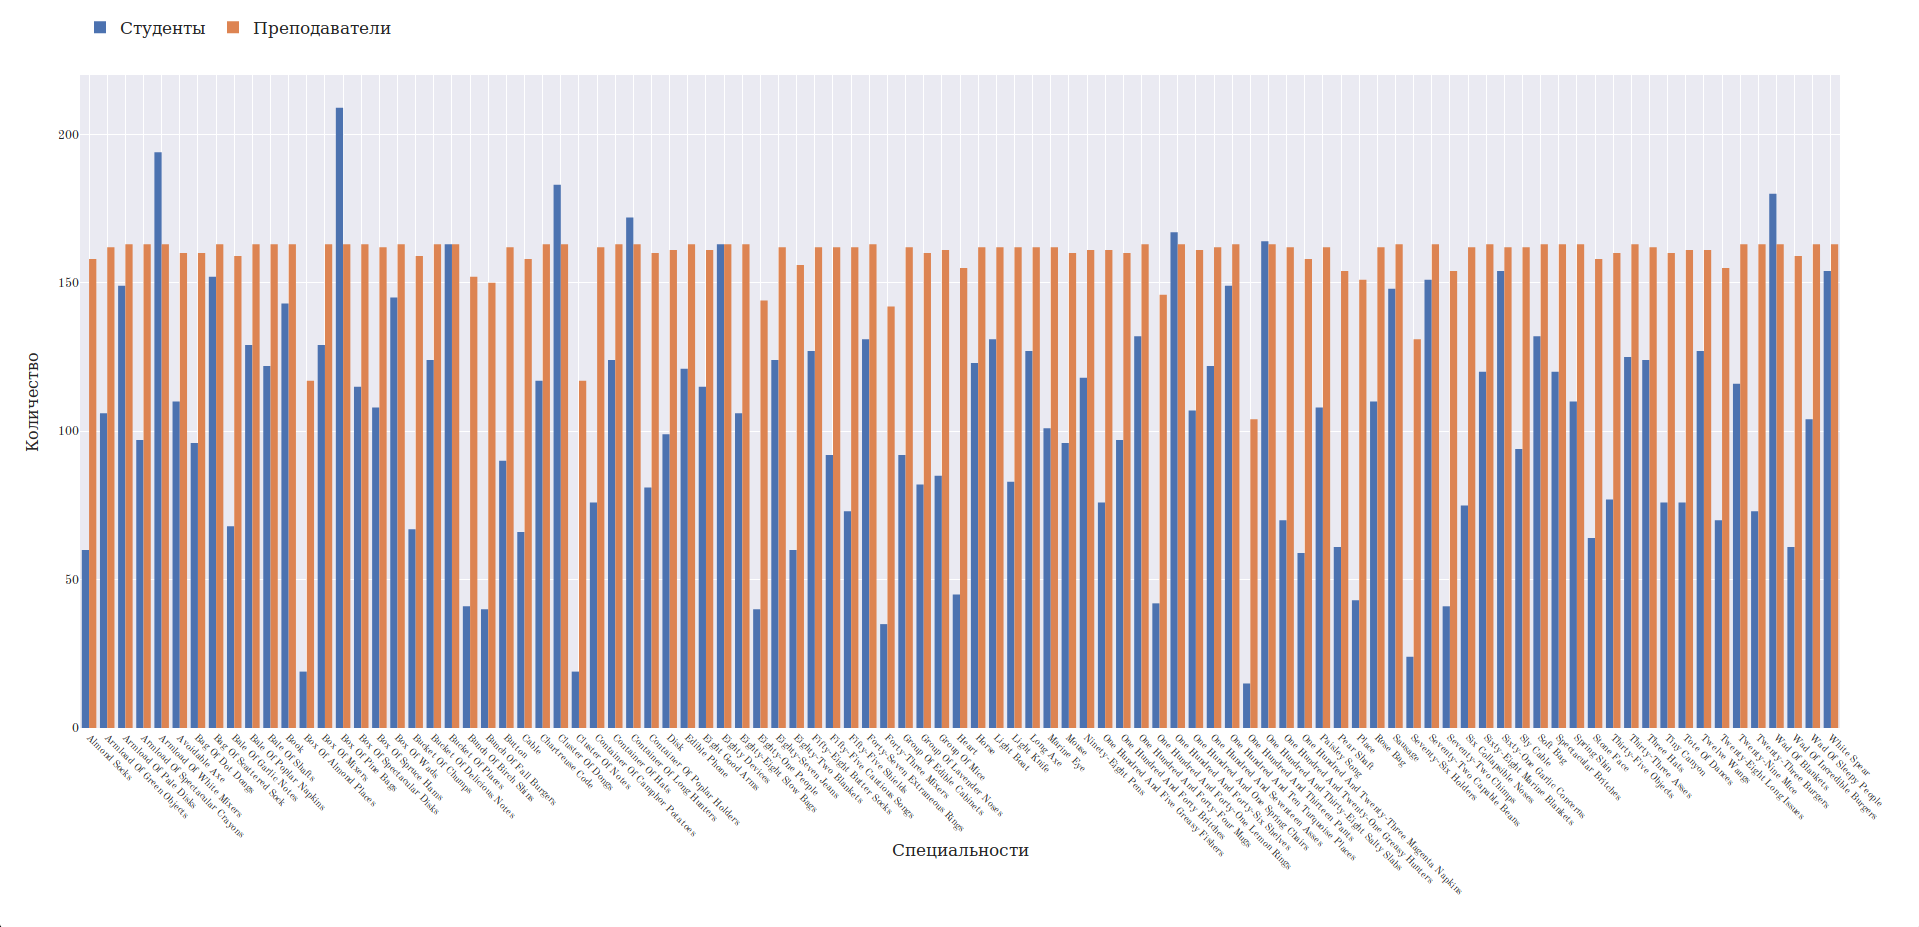
\includegraphics[width=26.5cm]{diagram}
    \caption{Да.}
\end{figure}
\end{landscape}

\subsection{Листинг}
\begin{code}
    \inputminted[breaklines=true, xleftmargin=1em,linenos, frame=single, framesep=10pt, firstline=1, lastline=33]{haskell}{listings/Parser.hs}
    \caption{Parser.hs --- функциональный код в массы!}
\end{code}

\section*{Заключение}
\LaTeX\ удобен для создания отчётов, так как сам следит за нумерацией таблиц, рисунков, листингов и отсылок к ним (так, например, здесь всегда будет указан номер рисунка "sample" не зависимо от того, какой он (1,2 или другой) - это рисунок \ref{pic:pic_name}). Не менее важно что весь документ оформлен в едином стиле, а исходные материалы подключаются к отчёту, а не хранятся в нём. Всё это позволяет легко получить качественный отчёт без дополнительных трат на его офрмление.

Исключения, пожалуй, составляют таблицы, так как их значительно сложнее создавать кодом, нежели в графическом редакторе. Но здесь никто не запрещает использовать визуальные средства создания таблиц для \LaTeX\ .
\addcontentsline{toc}{section}{Заключение}

% Не редактируем: Страница библиографии (формируется автоматически из книжек, указанных в refs.bib и пометок \cite{имя_источника} в тексте)
\newpage
\printbibliography[title=Перечень использованных источников]
\addcontentsline{toc}{section}{Перечень использованных источников}
\end{document}
